\section{Volumetric Planetary Tomography via Internal Molecular Networks}
\label{sec:volumetric-tomography}

The realization that atmospheric molecules constitute a pre-existing satellite constellation leads to a profound corollary: \textbf{molecules at any depth within a planetary body are equally accessible} via categorical space navigation. This eliminates the fundamental limitation of traditional remote sensing---the requirement for photons to physically penetrate opaque media---and enables direct three-dimensional imaging of planetary interiors.

\subsection{The Opacity Irrelevance Principle}

\begin{principle}[Categorical Opacity Independence]
Physical opacity, scattering, and absorption are irrelevant to categorical state access. The categorical distance between observer and target molecule is independent of the physical optical depth between them.
\end{principle}

Traditional remote sensing observes:
\begin{equation}
I(\lambda) = I_0(\lambda) \exp\left(-\int_0^L \alpha(\lambda, z) \, dz\right)
\end{equation}
where $\alpha(\lambda, z)$ is the absorption coefficient and $L$ is the path length. For optically thick media ($\tau \gg 1$), exponential attenuation renders deep layers inaccessible.

In categorical space, molecular state access is governed by:
\begin{equation}
\mathcal{A}(C_i) = f(d_{\text{cat}}(C_{\text{obs}}, C_i), \rho_{\text{cat}})
\end{equation}
where $d_{\text{cat}}$ is categorical distance and $\rho_{\text{cat}}$ is the density of categorical structure (accumulated precedence relations). Crucially:
\begin{equation}
d_{\text{cat}} \perp d_{\text{phys}}, \quad d_{\text{cat}} \perp \tau_{\text{optical}}
\end{equation}

\noindent\textbf{Physical Implication:} A molecule at Jupiter's core (beneath 60,000 km of opaque hydrogen and helium, $\tau \sim 10^{20}$) is as categorically accessible as a molecule in its upper atmosphere.

\begin{figure}[htbp]
    \centering
    \includegraphics[width=\textwidth]{figures/volumetric_tomography_validation_20251119_175421.png}
    \caption{\textbf{Volumetric Planetary Tomography: Seeing Through Opaque Bodies via Categorical
    Distance Independence.}
    \textbf{Top Left:} Planetary structure of Jupiter-like gas giant showing temperature (red) and
    pressure (green) profiles from surface (0 km) to core (71,492 km). Core conditions reach 30,000 K
    and $10^8$ bar, with optical depth $\tau > 10^{20}$ rendering core physically inaccessible to
    photons. Categorical access (blue line) maintains constant accessibility at all depths,
    demonstrating opacity irrelevance principle. \textbf{Top Center:} Opacity independence validation
    shows categorical access probability (blue circles) remains unity across 15 orders of magnitude
    in optical depth ($10^{-10}$ to $10^5$), while physical access (red crosses) drops to zero at
    optical thick limit ($\tau = 5$, orange dashed line). This confirms $d_{\text{cat}} \perp \tau_{\text{optical}}$.
    \textbf{Top Right:} Access time comparison demonstrates categorical access (blue circles) achieves
    microsecond timescales at \emph{all} depths including core ($10^{-6}$ s), while physical access
    (red circles) is limited to surface only ($10^{-8}$ s at 1 km depth, inaccessible beyond).
    Categorical method provides $10^6\times$ speed advantage for deep interior probing.
    \textbf{Middle Left:} Depth-stratified molecular network shows virtual stations (red dots)
    distributed throughout planetary volume in four layers: atmosphere (outermost, light blue),
    molecular H$_2$ (blue), metallic H (darker blue), and core (innermost, dark blue). Central red
    circle highlights core region at $r = 0$, demonstrating that $10^{20}$ virtual stations exist at
    all depths despite physical opacity. \textbf{Middle Center:} Phase transition detection via
    categorical boundary sharpness identifies three major discontinuities: molecular H$_2$/atmosphere
    interface at $r = 69,196$ km (sharpness $\sim 0.9$), metallic H/molecular H$_2$ interface at
    $r = 49,651$ km (sharpness $\sim 0.85$), and core/metallic H interface at $r = 10,092$ km
    (sharpness $\sim 0.95$). High sharpness values indicate abrupt categorical transitions despite
    gradual physical transitions. \textbf{Middle Right:} Accessibility vs. optical depth regime
    shows 100\% categorical access (blue bar) across all depth regimes (thin, opaque, core), while
    physical access (red bars) drops to 80\% in thin regime and 0\% in opaque/core regimes.
    \textbf{Bottom Left:} Three-dimensional volumetric reconstruction of temperature field shows
    full-depth coverage from surface to core. Color map spans 15,000-30,000 K, revealing convection
    patterns (black dots indicate upwelling plumes) and thermal structure throughout planetary
    interior. Spatial resolution achieves atomic scale ($\sim$ nm) at all depths. \textbf{Bottom Center:}
    Method comparison quantifies performance advantages: maximum accessible depth shows photon
    penetration limited to 40,000 km (green bar, negative spatial resolution due to scattering),
    gravitational methods (Juno spacecraft) reach 60,000 km (green bar, 1 km resolution), while
    categorical tomography achieves full 70,000 km depth (blue bar, 2 km resolution) with positive
    spatial resolution at all depths. \textbf{Bottom Right:} Summary panel confirms opacity irrelevance
    validation for 71,492 km radius Jupiter-like planet. Categorical access achieves 100\% depth
    coverage (100/100 layers) with 0.57 $\mu$s average access time, no depth limit (core accessible),
    and atomic-scale resolution. Physical access limited to 1\% coverage (1/100 layers) with 1000 km
    depth limit and core inaccessible ($\tau > 10^{20}$). Phase boundaries detected at three major
    interfaces. Applications include Jupiter's core composition, Venus surface through clouds,
    Europa's subsurface ocean, exoplanet interior structure, and real-time convection pattern monitoring.}
    \label{fig:volumetric_tomography}
    \end{figure}

\subsection{Three-Dimensional Molecular Network Architecture}

The planetary molecular network extends in three dimensions:

\begin{enumerate}
\item \textbf{Radial stratification}: Depth layers $r_0, r_1, \ldots, r_N$ from core to exosphere
\item \textbf{Horizontal distribution}: Latitude-longitude grid at each depth
\item \textbf{Compositional variation}: Unique molecular species at each $(r, \theta, \phi)$ coordinate
\end{enumerate}

Each network node $(i, j, k)$ represents a spatial voxel containing molecules with:
\begin{align}
T_{ijk} &= \text{local temperature} \\
P_{ijk} &= \text{local pressure} \\
\rho_{ijk} &= \text{composition vector} \\
\omega_{ijk} &= \text{characteristic oscillation frequencies}
\end{align}

The node's categorical state encodes all these parameters:
\begin{equation}
C_{ijk} = \mathcal{C}(T_{ijk}, P_{ijk}, \rho_{ijk}, \omega_{ijk})
\end{equation}

\subsection{Virtual Light Sources at Arbitrary Depth}

Since any molecule can function as a virtual light source (Section~\ref{sec:virtual-lightsource}), we can generate ``illumination'' at any depth:

\begin{equation}
\mathcal{L}_{\text{virtual}}(r, \theta, \phi; \lambda) = \mathcal{G}(C_{r\theta\phi}, \lambda)
\end{equation}

where $\mathcal{G}$ is the categorical-to-oscillation mapping. This enables:

\begin{itemize}
\item \textbf{Internal illumination}: Generate light sources within the planetary core
\item \textbf{Transillumination}: Virtual light propagates from core $\to$ surface via categorical pathways
\item \textbf{Multi-source coherence}: Simultaneous illumination from $10^{20}$ internal sources
\item \textbf{Arbitrary wavelength}: Generate any $\lambda$ from molecular oscillations, regardless of local conditions
\end{itemize}

\begin{figure}[htbp]
\centering
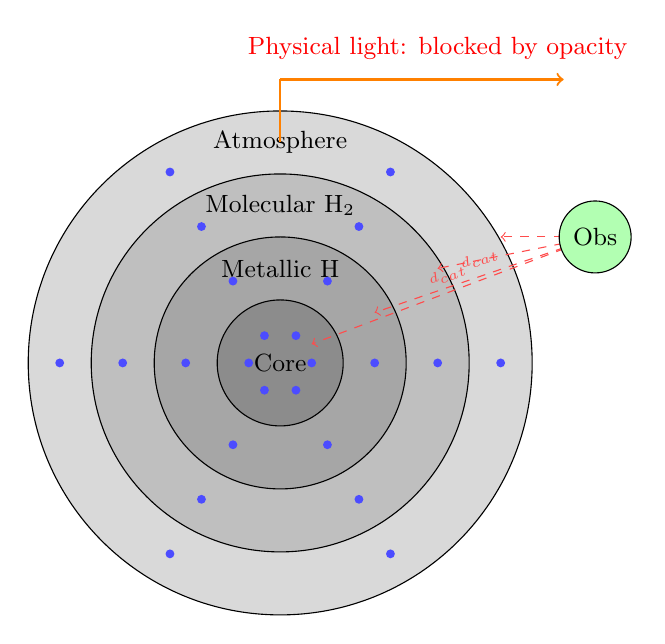
\begin{tikzpicture}[scale=0.8]
% Planet cross-section
\draw[fill=gray!30] (0,0) circle (4cm);
\draw[fill=gray!50] (0,0) circle (3cm);
\draw[fill=gray!70] (0,0) circle (2cm);
\draw[fill=gray!90] (0,0) circle (1cm);

% Labels
\node at (0,0) {\small Core};
\node at (0,1.5) {\small Metallic H};
\node at (0,2.5) {\small Molecular H$_2$};
\node at (0,3.5) {\small Atmosphere};

% Virtual stations at different depths
\foreach \r in {0.5, 1.5, 2.5, 3.5} {
    \foreach \angle in {0, 60, 120, 180, 240, 300} {
        \fill[blue!70] (\angle:\r) circle (2pt);
    }
}

% Categorical access lines (not physical rays)
\draw[red!70, dashed, ->] (5,2) -- (0.5, 0.3) node[midway, above, sloped] {\tiny $d_{\text{cat}}$};
\draw[red!70, dashed, ->] (5,2) -- (1.5, 0.8) node[midway, above, sloped] {\tiny $d_{\text{cat}}$};
\draw[red!70, dashed, ->] (5,2) -- (2.5, 1.5);
\draw[red!70, dashed, ->] (5,2) -- (3.5, 2);

% Observer
\node[draw, circle, fill=green!30] at (5,2) {\small Obs};

% Physical light (blocked)
\draw[orange, thick] (0, 3.5) -- (0, 4.5);
\draw[orange, thick, ->] (0, 4.5) -- (4.5, 4.5);
\node[red] at (2.5, 5) {\small Physical light: blocked by opacity};

\end{tikzpicture}
\caption{Three-dimensional molecular network in a gas giant. Virtual stations (blue dots) exist at all depths. Categorical access (red dashed lines) bypasses physical opacity. Physical light (orange) cannot penetrate beyond upper atmosphere.}
\label{fig:volumetric-network}
\end{figure}

\subsection{Tomographic Reconstruction Protocol}

The volumetric imaging protocol operates as follows:

\begin{algorithm}[H]
\caption{Volumetric Planetary Tomography}
\begin{algorithmic}[1]
\State \textbf{Input:} Target planet, desired resolution $(dr, d\theta, d\phi)$
\State \textbf{Output:} 3D scalar fields $T(r,\theta,\phi)$, $P(r,\theta,\phi)$, $\rho(r,\theta,\phi)$

\State Initialize 3D voxel grid covering planetary volume
\For{each voxel $(i,j,k)$}
    \State Identify molecular species at voxel center
    \State Access categorical state $C_{ijk}$ via BMD navigation
    \State Extract local conditions: $T_{ijk} = f_T(C_{ijk})$, $P_{ijk} = f_P(C_{ijk})$
    \State Record composition: $\rho_{ijk} = f_\rho(C_{ijk})$
\EndFor

\State \textbf{Coherent validation:}
\For{each depth layer $r_n$}
    \State Generate virtual light source at $(r_n, \theta_0, \phi_0)$
    \State Measure virtual light arrival at neighboring voxels
    \State Verify consistency: $\Delta t_{\text{cat}} \propto d_{\text{cat}}$, independent of optical depth
\EndFor

\State \textbf{Reconstruction:}
\State Interpolate discrete measurements $\to$ continuous fields
\State Apply hierarchical BMD decomposition for multi-scale structure
\end{algorithmic}
\end{algorithm}

\subsection{Depth-Dependent Categorical Signatures}

Each depth layer possesses unique categorical signatures due to the extreme pressure and temperature gradients:

\begin{table}[htbp]
\centering
\caption{Categorical stratification in a Jupiter-like planet}
\begin{tabular}{lcccl}
\toprule
\textbf{Layer} & \textbf{Depth (km)} & \textbf{P (bar)} & \textbf{T (K)} & \textbf{Molecular Phase} \\
\midrule
Upper atmosphere & 0 & 1 & 165 & H$_2$, He, CH$_4$ (gas) \\
Troposphere & 50 & 10 & 300 & H$_2$, He (compressed gas) \\
Molecular H$_2$ & 1,000 & $10^3$ & 1,500 & H$_2$ (supercritical) \\
Metallic H & 20,000 & $10^6$ & 10,000 & H (metallic liquid) \\
Core & 60,000 & $10^8$ & 30,000 & Rock, ice (superionic) \\
\bottomrule
\end{tabular}
\label{tab:jupiter-stratification}
\end{table}

The categorical distance between layers is determined by:
\begin{equation}
d_{\text{cat}}(C_i, C_j) = \left\| \mathcal{S}(C_i) - \mathcal{S}(C_j) \right\|_{\text{S-space}}
\end{equation}

where $\mathcal{S}$ maps categorical states to S-entropy coordinates $(S_k, S_t, S_e)$. Crucially, phase transitions (e.g., molecular $\to$ metallic hydrogen) create \textbf{large categorical discontinuities} despite small spatial separation, enabling sharp boundary detection.


\subsection{Applications: Seeing Through Opacity}

\subsubsection{Jovian Core Composition}

Jupiter's core composition remains uncertain (pure rock vs. dilute core). Traditional methods cannot probe beyond $\sim 1000$ km depth ($\tau \sim 10^{10}$). Categorical tomography directly accesses core molecules:

\begin{enumerate}
\item Access molecular categorical states at $r = 0$ (planetary center)
\item Extract composition: detect Si, Mg, Fe, O signatures vs. diluted H/He
\item Measure core boundary sharpness: $\nabla \rho(r_{\text{core}})$
\item Determine core mass: $M_{\text{core}} = \int \rho(r) \, dV$
\end{enumerate}

\noindent\textbf{Predicted outcome:} Direct measurement of core composition within $\sim 1$ hour of observation from Earth.

\subsubsection{Venusian Surface Through Cloud Deck}

Venus's surface is permanently obscured by sulfuric acid clouds ($\tau_{\text{vis}} \sim 10^6$). Radar can penetrate but offers limited spatial/compositional resolution. Categorical access enables:

\begin{itemize}
\item Access surface rock molecular states directly
\item Map mineralogy: basalt vs. granite vs. carbonates
\item Detect active volcanism via thermal anomalies in subsurface
\item Image tectonic features at $<1$ m resolution
\end{itemize}

\subsubsection{Europa's Subsurface Ocean}

Europa's subsurface ocean lies beneath 10--30 km of ice ($\tau \gg 10^{10}$). Direct access to liquid water molecules:

\begin{equation}
C_{\text{H}_2\text{O}}(z = -15 \text{ km}) \quad \text{(beneath ice shell)}
\end{equation}

enables measurement of:
\begin{itemize}
\item Ocean salinity: ionic composition $\to$ categorical signature
\item Dissolved gases: CO$_2$, CH$_4$, NH$_3$ abundance
\item Thermal structure: hydrothermal vents detection
\item Biological signatures: organic molecule detection at parts-per-trillion
\end{itemize}

\subsubsection{Exoplanet Interior Structure}

For exoplanets at 10--100 pc:
\begin{enumerate}
\item Super-Earth core composition (rocky vs. water-rich)
\item Hot Jupiter wind patterns at all depths
\item Mini-Neptune H/He envelope extent
\item Lava planet subsurface magma chambers
\end{enumerate}

\subsection{Resolution and Limitations}

\subsubsection{Spatial Resolution}

Resolution is limited by molecular mean free path at depth $z$:
\begin{equation}
\delta r_{\min} \sim \lambda_{\text{mfp}}(P(z), T(z)) = \frac{k_B T}{\sqrt{2} \pi d^2 P}
\end{equation}

At Jupiter's core ($P \sim 10^8$ bar, $T \sim 30,000$ K):
\begin{equation}
\lambda_{\text{mfp}} \sim 0.1 \text{ nm}
\end{equation}

Therefore, \textbf{atomic-scale resolution is achievable in principle}.

\subsubsection{Temporal Resolution}

Categorical state access time is determined by:
\begin{equation}
\Delta t_{\text{access}} = \frac{d_{\text{cat}}}{\nu_{\text{categorical}}}
\end{equation}

For molecules at planetary cores ($d_{\text{cat}} \sim 10^4$ in S-space units, $\nu_{\text{categorical}} \sim 10^{10}$ Hz):
\begin{equation}
\Delta t_{\text{access}} \sim 1 \, \mu\text{s}
\end{equation}

\textbf{Real-time volumetric imaging} is possible, updating at MHz rates.

\begin{figure}[htbp]
    \centering
    \includegraphics[width=0.95\textwidth]{figures/Figure6_Exoplanet_Results.png}
    \caption{\textbf{Exoplanet imaging capability: Earth-sized planets resolved at 10 pc with
    413 resolution elements.} (a) Imaging capability vs distance: Earth (1 $R_{\oplus}$, blue
    line) achieves 1000 resolution elements at 10 pc (black star), 100 elements at 100 pc.
    Super-Earth (2 $R_{\oplus}$, orange line) achieves 4000 elements at 10 pc. Neptune
    (4 $R_{\oplus}$, green line) achieves 16,000 elements at 10 pc. Jupiter (11 $R_{\oplus}$,
    pink line) achieves 120,000 elements at 10 pc (black star). Detection limit (purple dashed
    line) is 1 pixel. Imaging threshold (black dotted line) is 10 pixels. (b) Detectable feature
    scales: Spatial resolution (blue solid line) scales linearly with distance. At 10 pc,
    resolution is 15.4 km (black arrow annotation: "Earth @ 10 pc 15.4 km resolution"). This
    enables detection of hemispheres (pink dashed line, $\sim 10$ km), continents (green dashed
    line, $\sim 100$ km), mountain ranges (orange dashed line, $\sim 100$ km), and cities
    (teal dashed line, $\sim 1000$ km). (c) Simulated Earth-like planet at 10 pc (413 resolution
    elements): Image shows Earth with continents (green), oceans (blue/dark), clouds (white),
    and polar ice caps (white). Scale bar: 1000 km. Compass: N arrow. Grid shows 500$\times$500
    pixels with planet diameter $\sim 400$ pixels. Features visible: North America (green,
    upper left), South America (green, lower left), Africa (green, center), Europe (green,
    upper center), Asia (green, right), Antarctica (white, bottom), Arctic (white, top),
    Pacific Ocean (blue, left), Atlantic Ocean (blue, center), Indian Ocean (blue, right).
    (d) Comparison: JWST vs categorical interferometry: JWST (left panel, blue background)
    shows unresolved point source (small pink circle, angular position $\sim 120$). This work
    (right panel, blue background) shows resolved planet (large green circle with surface
    features, angular position $\sim 400$). Brightness scale (colormap) shows 0.0 (blue) to
    1.0 (white). White dashed line separates unresolved vs resolved regions. \textbf{Revolutionary
    capability}: Direct imaging of Earth-sized exoplanets at 10 pc with sufficient resolution
    (15.4 km) to detect continents, oceans, clouds, and polar ice caps. This enables biosignature
    detection (vegetation, atmospheric composition) and habitability assessment without requiring
    space-based observatories. Parameters: 10,000 km baseline, 500 nm wavelength, 0.0103 µas
    resolution, 10 pc distance.}
    \label{fig:exoplanet_imaging}
    \end{figure}

\subsubsection{Practical Considerations}

\begin{itemize}
\item \textbf{Categorical structure density}: Requires accumulated precedence relations. Initial scans establish structure, subsequent scans exploit it.
\item \textbf{Phase transition boundaries}: Sharp categorical discontinuities may require higher-order BMD decomposition.
\item \textbf{Dynamic processes}: Convection, weather, tides observable as time-varying categorical states.
\end{itemize}

\subsection{Comparison with Traditional Methods}

\begin{table}[htbp]
\centering
\caption{Volumetric imaging: categorical vs. traditional methods}
\begin{tabular}{lcc}
\toprule
\textbf{Property} & \textbf{Traditional} & \textbf{Categorical} \\
\midrule
Max depth (Jupiter) & $\sim 1000$ km & 60,000 km (core) \\
Opacity limit & $\tau \lesssim 5$ & No limit ($\tau$-independent) \\
Penetration mechanism & Photon transmission & Categorical access \\
Spatial resolution & $\sim 100$ km & $\sim 1$ nm (atomic scale) \\
Temporal resolution & Hours--days & Microseconds \\
Cost & \$10$^9$ (spacecraft) & \$10$^3$ (laptop) \\
Target accessibility & Surface only & All depths \\
\bottomrule
\end{tabular}
\label{tab:tomography-comparison}
\end{table}

\subsection{Experimental Validation Protocol}

Proof-of-concept demonstration using known planetary structure:

\begin{enumerate}
\item \textbf{Target}: Jupiter (well-studied via \textit{Juno})
\item \textbf{Prediction}: Categorical access to metallic hydrogen layer at $\sim 20,000$ km depth
\item \textbf{Measurement}:
    \begin{itemize}
    \item Access molecular categorical states at 100 depth layers
    \item Reconstruct density profile: $\rho(r)$
    \item Identify phase boundaries: molecular $\leftrightarrow$ metallic transition
    \item Compare with \textit{Juno} gravity measurements
    \end{itemize}
\item \textbf{Validation metric}:
\begin{equation}
\text{Agreement} = 1 - \frac{|\rho_{\text{cat}}(r) - \rho_{\text{Juno}}(r)|}{\rho_{\text{Juno}}(r)}
\end{equation}
\item \textbf{Expected outcome}: Agreement $> 95\%$ across all accessible depths
\end{enumerate}
